
\chapter{Resultados}

\section{Desempenho geral do modelo}

Após o treinamento da regressão linear múltipla, foram avaliadas as métricas de desempenho nos conjuntos de treino e teste. O modelo apresentou coeficiente de determinação ($R^2$) de 0,3512 no treino e 0,3625 no teste, indicando que aproximadamente 35,12\% e 36,25\% da variabilidade do consumo de energia elétrica, respectivamente, são explicadas pelas variáveis utilizadas.

A proximidade entre os valores de $R^2$ dos dois conjuntos indica que o modelo apresentou comportamento semelhante nos dados utilizados durante o treinamento e nos dados não utilizados nessa etapa. Portanto, não há evidência significativa de sobreajuste.

Em relação aos erros, o MAE foi de 3486,69 kWh no treino e 3421,56 kWh no teste, enquanto o RMSE foi de 4488,82 kWh e 4412,00 kWh, respectivamente. Esses valores indicam que as previsões ainda apresentam diferenças consideráveis em relação aos consumos observados.

A validação cruzada com cinco partições apresentou $R^2$ médio de 0,3523, com desvio padrão de 0,0053. A baixa variação entre as partições indica estabilidade no desempenho do modelo diante de diferentes divisões dos dados.

\section{Relação entre as variáveis}

A matriz de correlação permite observar a intensidade e a direção das relações lineares entre as variáveis preditoras e o consumo de energia elétrica.

\begin{figure}[htbp]
	\centering
	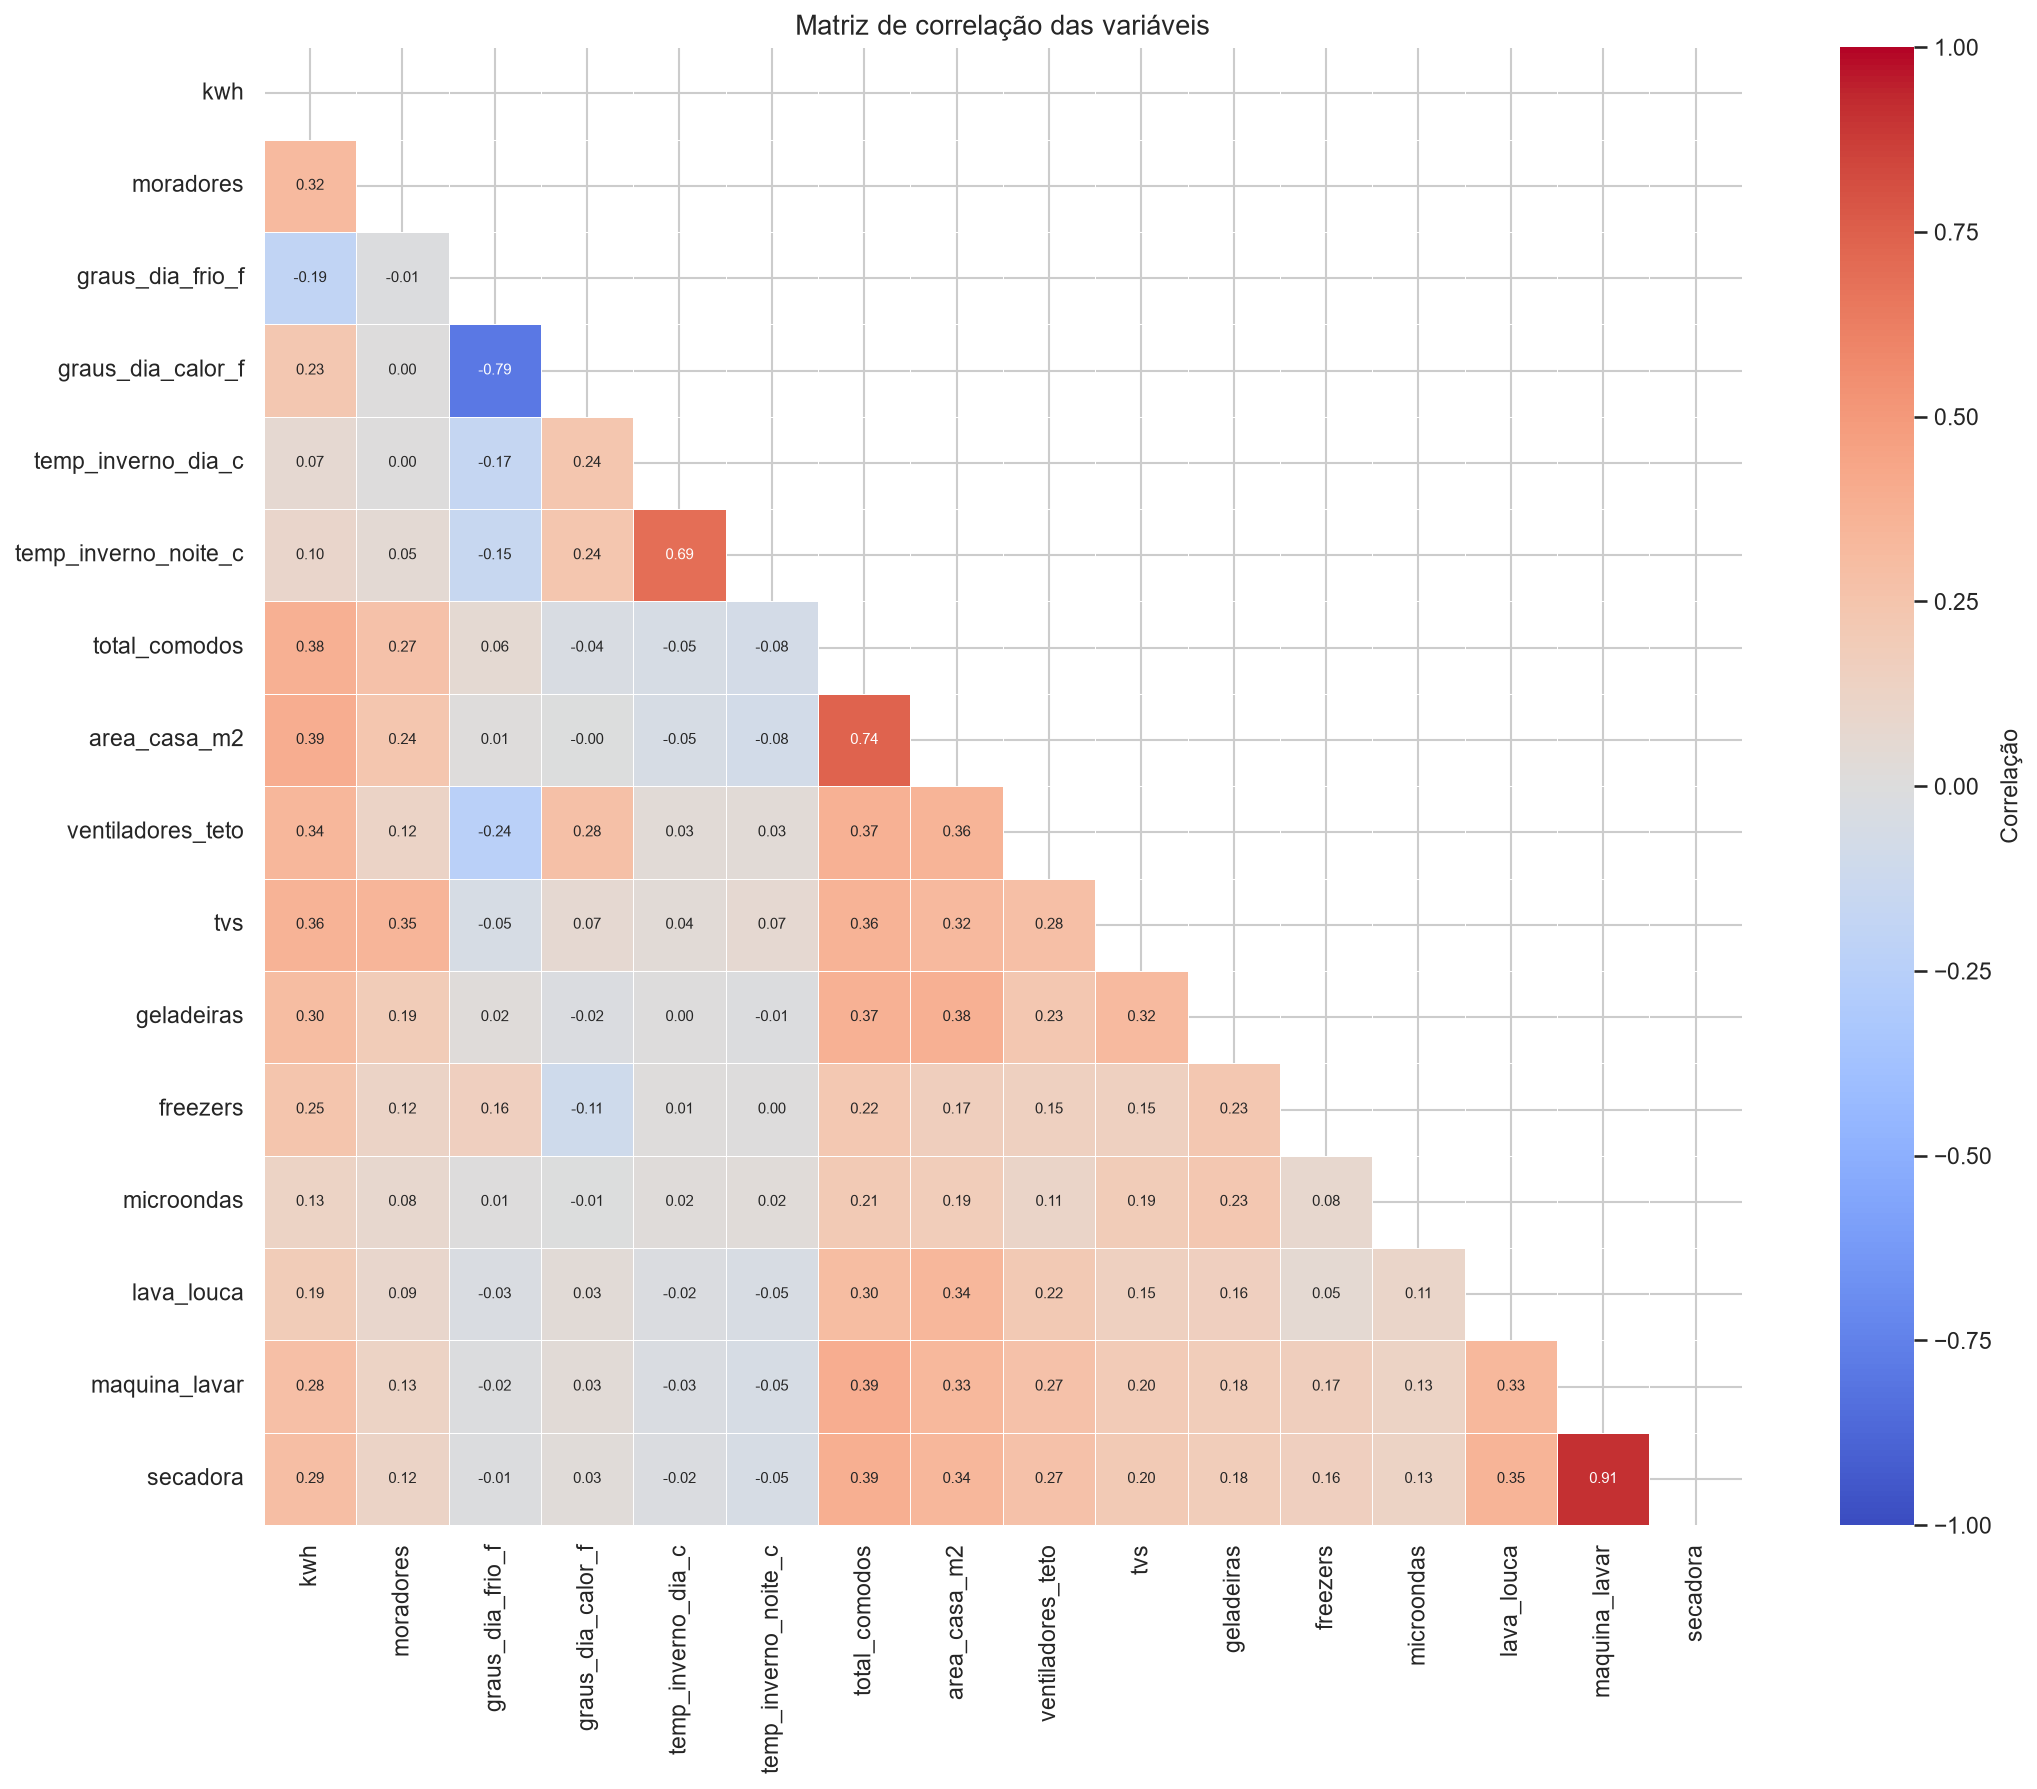
\includegraphics[width=0.95\textwidth]{figuras/01_matriz_correlacao.png}
	\caption{Matriz de correlação entre as variáveis do conjunto de dados.}
	\label{fig:correlacao}
\end{figure}

Conforme observado na matriz, as variáveis apresentam diferentes níveis de correlação com o consumo. A área da residência destaca-se entre as variáveis com maior correlação positiva, conforme também discutido na metodologia. Entretanto, nenhuma variável isolada apresenta correlação suficiente para explicar a maior parte da variação do consumo, reforçando a utilização de múltiplas variáveis no modelo.

Para complementar essa análise, foram gerados gráficos de dispersão relacionando individualmente cada variável preditora com o consumo de energia elétrica.

\begin{figure}[htbp]
	\centering
	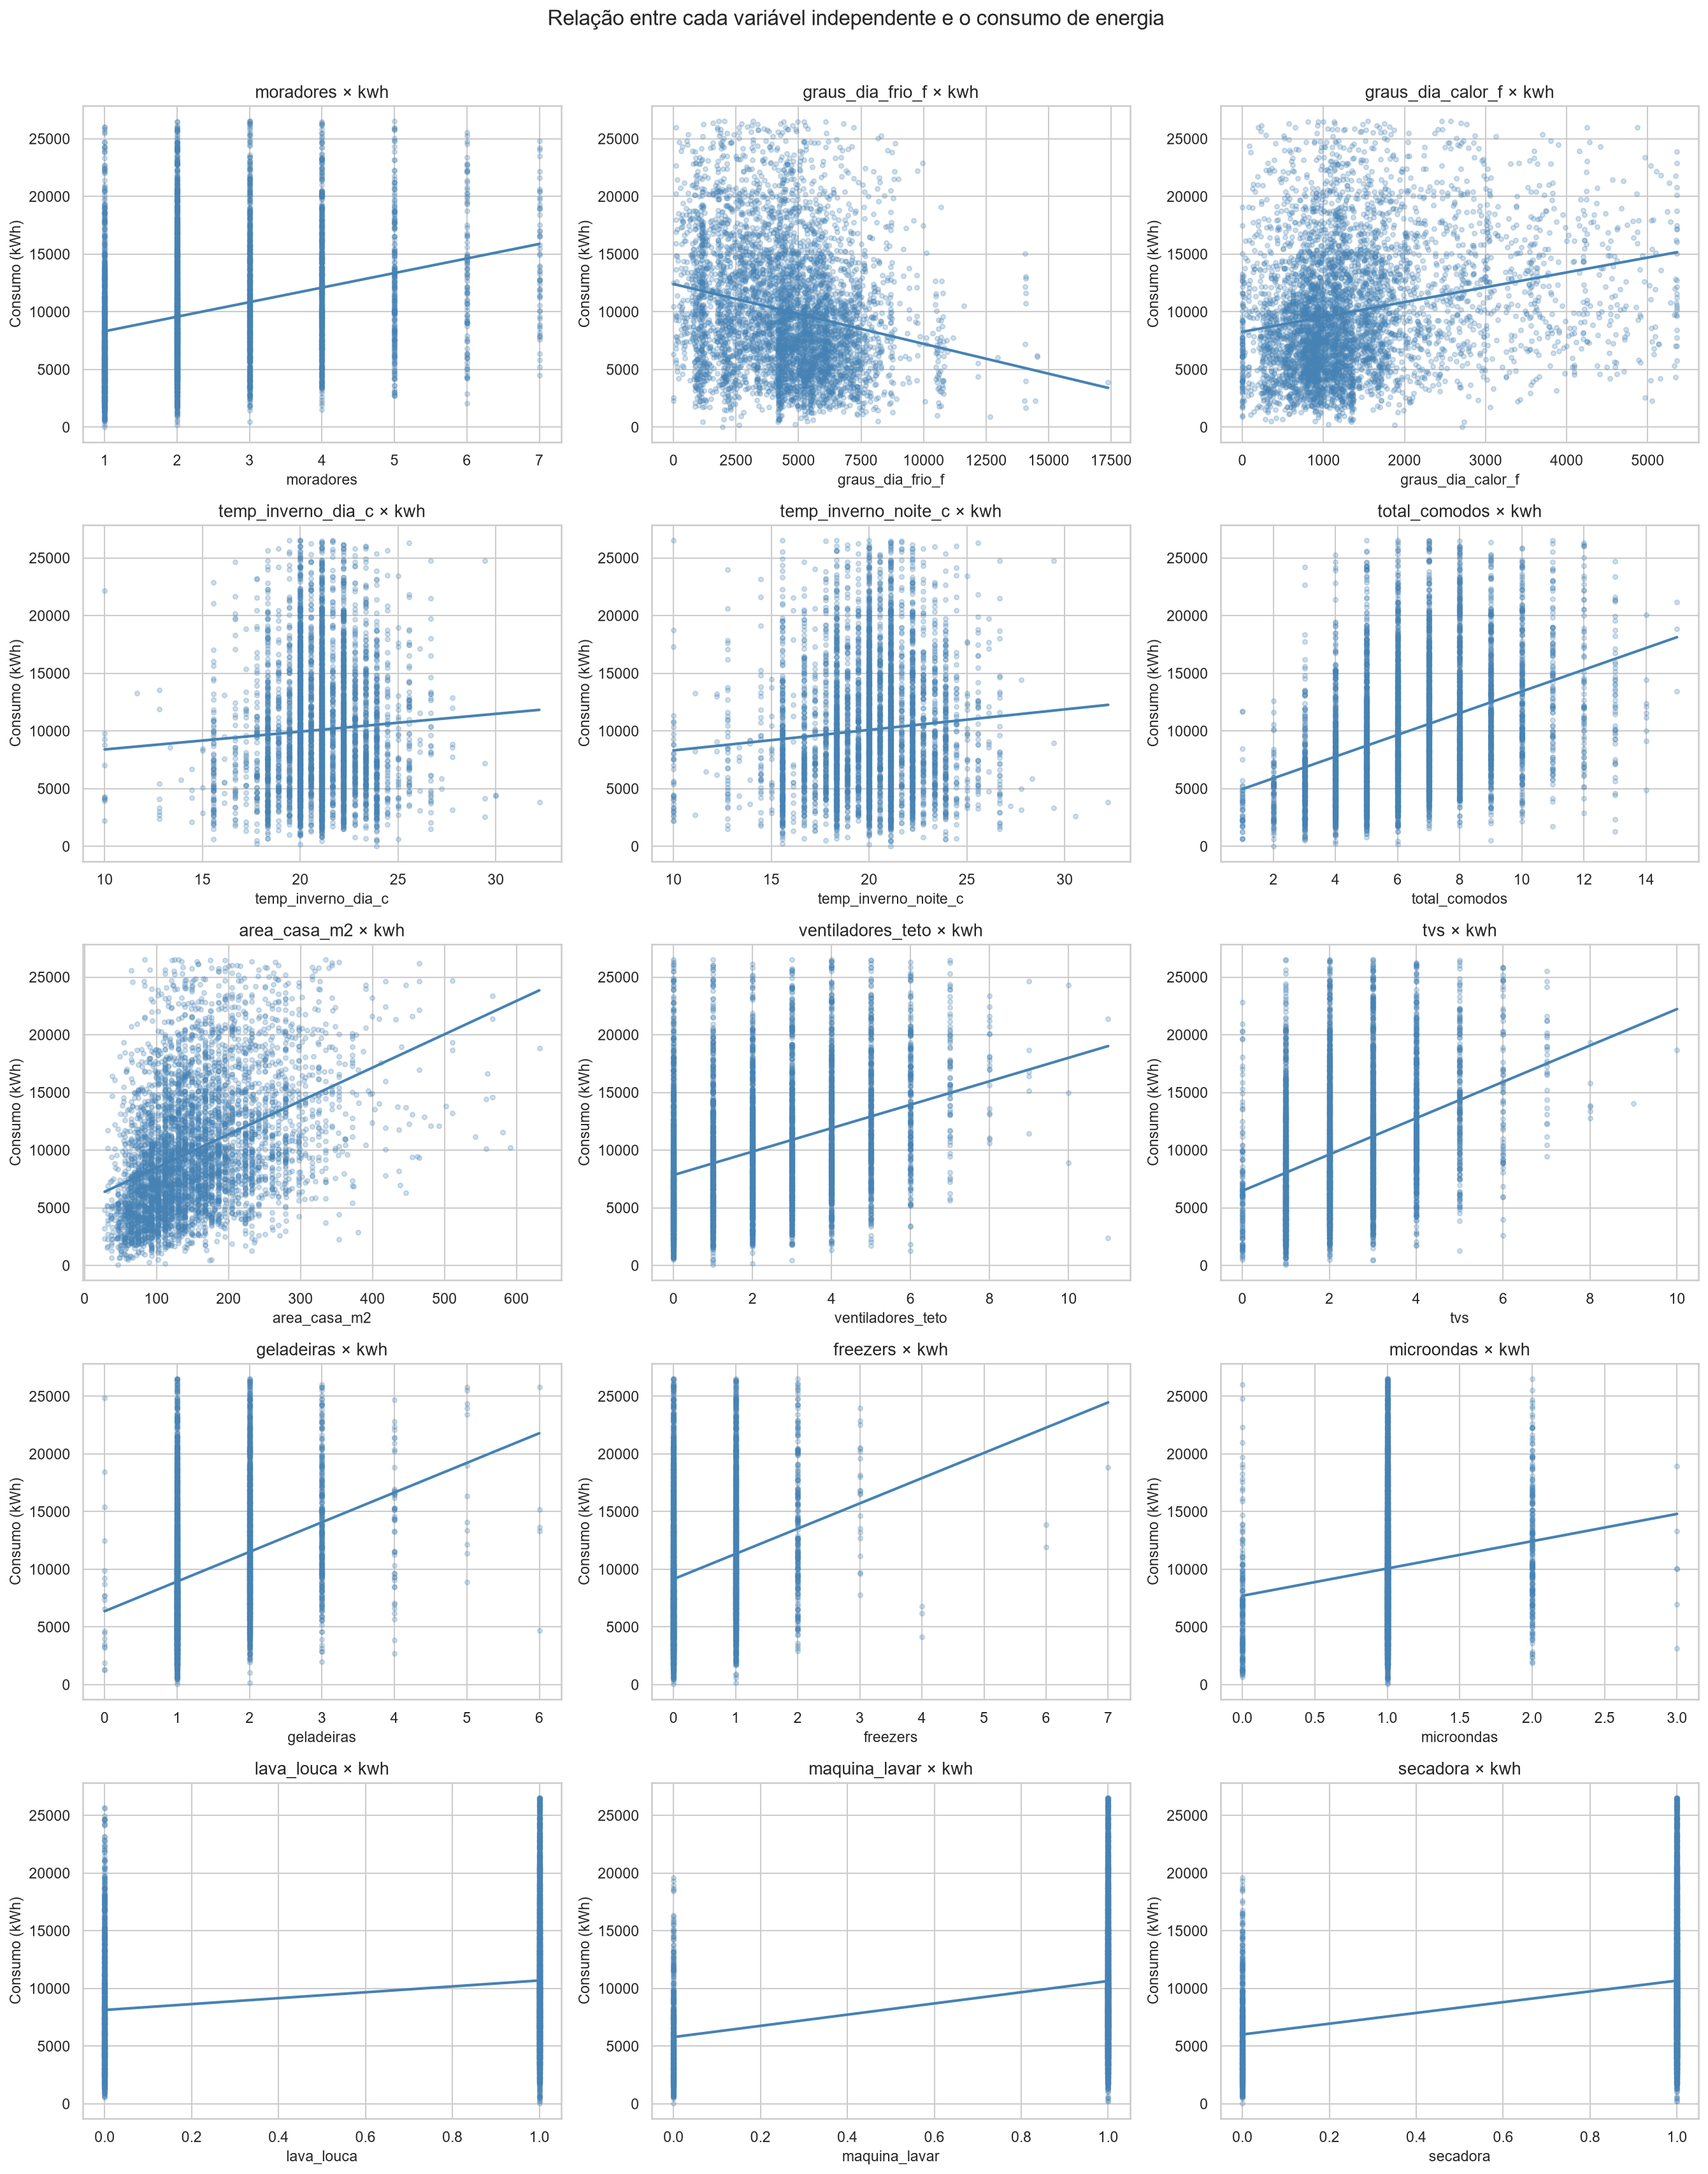
\includegraphics[width=\textwidth]{figuras/02_dispersao_variaveis_kwh.png}
	\caption{Gráficos de dispersão das variáveis preditoras em relação ao consumo de energia elétrica.}
	\label{fig:dispersao}
\end{figure}

Os gráficos permitem visualizar tendências individuais entre as características dos domicílios e o consumo. As linhas de tendência representam ajustes lineares simples entre cada variável e o consumo, não correspondendo diretamente ao hiperplano estimado pela regressão múltipla. Dessa forma, essas visualizações auxiliam na compreensão dos dados, mas não devem ser interpretadas isoladamente como o comportamento completo do modelo.

\section{Comparação entre valores reais e previstos}

Para avaliar visualmente a capacidade preditiva do modelo, foram comparados os valores reais e previstos de consumo no conjunto de teste. A linha diagonal representa a situação ideal, na qual os valores previstos seriam exatamente iguais aos observados.

\begin{figure}[htbp]
	\centering
	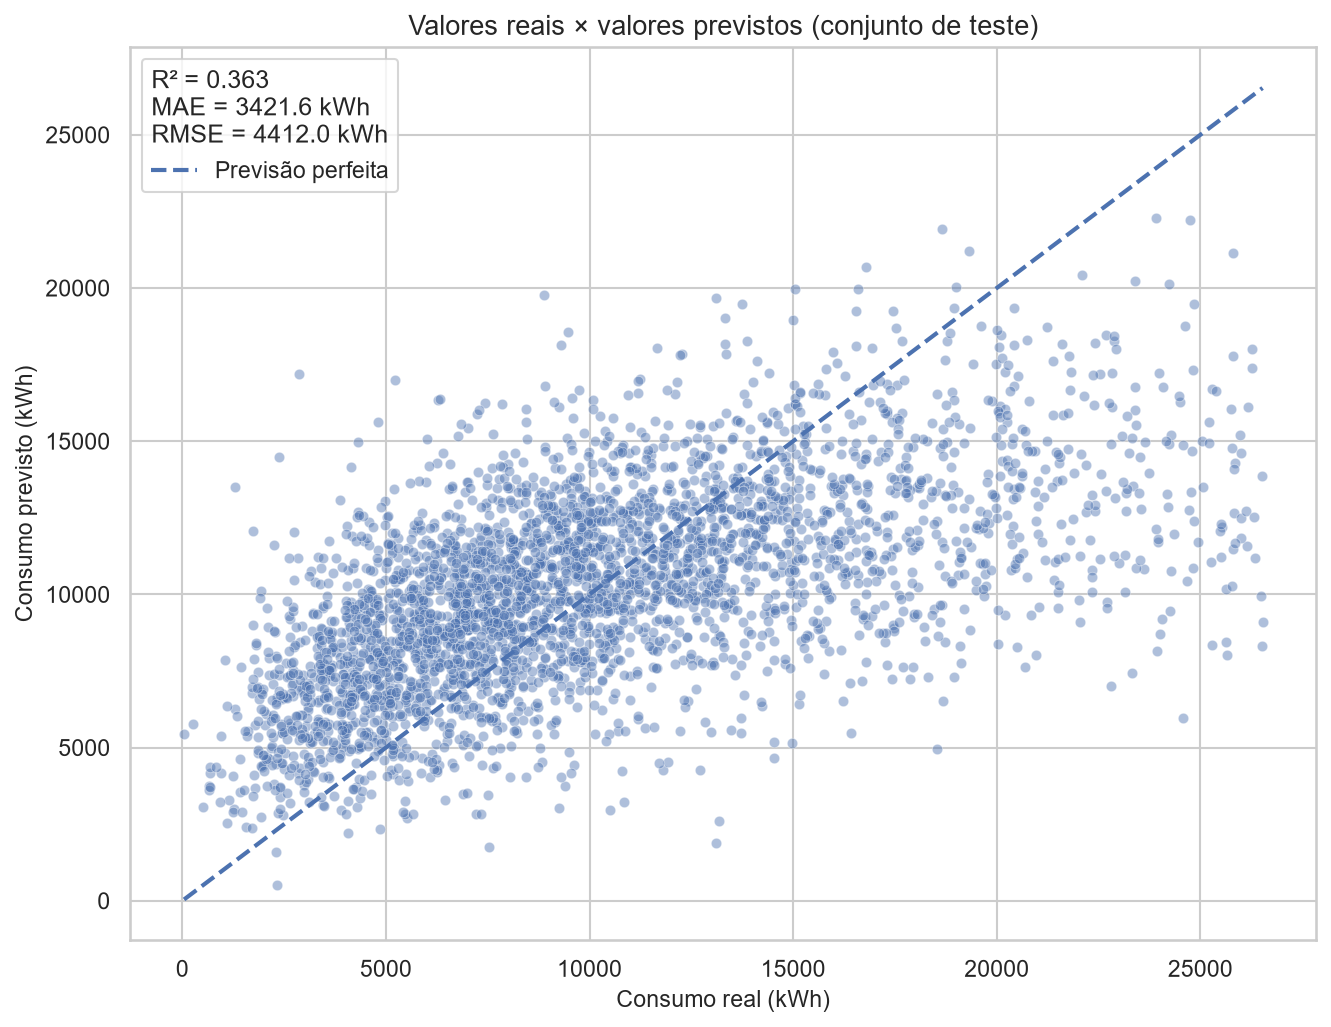
\includegraphics[width=0.85\textwidth]{figuras/03_valores_reais_vs_previstos.png}
	\caption{Comparação entre os valores reais e previstos de consumo no conjunto de teste.}
	\label{fig:real_previsto}
\end{figure}

A distribuição dos pontos em relação à linha de referência permite observar a proximidade entre as previsões e os valores reais. Embora exista uma tendência de acompanhamento dos valores observados, a dispersão dos pontos indica que o modelo ainda apresenta erros consideráveis, resultado compatível com o coeficiente de determinação obtido.

\section{Análise dos resíduos}

Os resíduos correspondem à diferença entre o consumo real e o consumo previsto pelo modelo. Valores positivos representam situações em que o modelo subestimou o consumo, enquanto valores negativos indicam superestimação.

\begin{figure}[htbp]
	\centering
	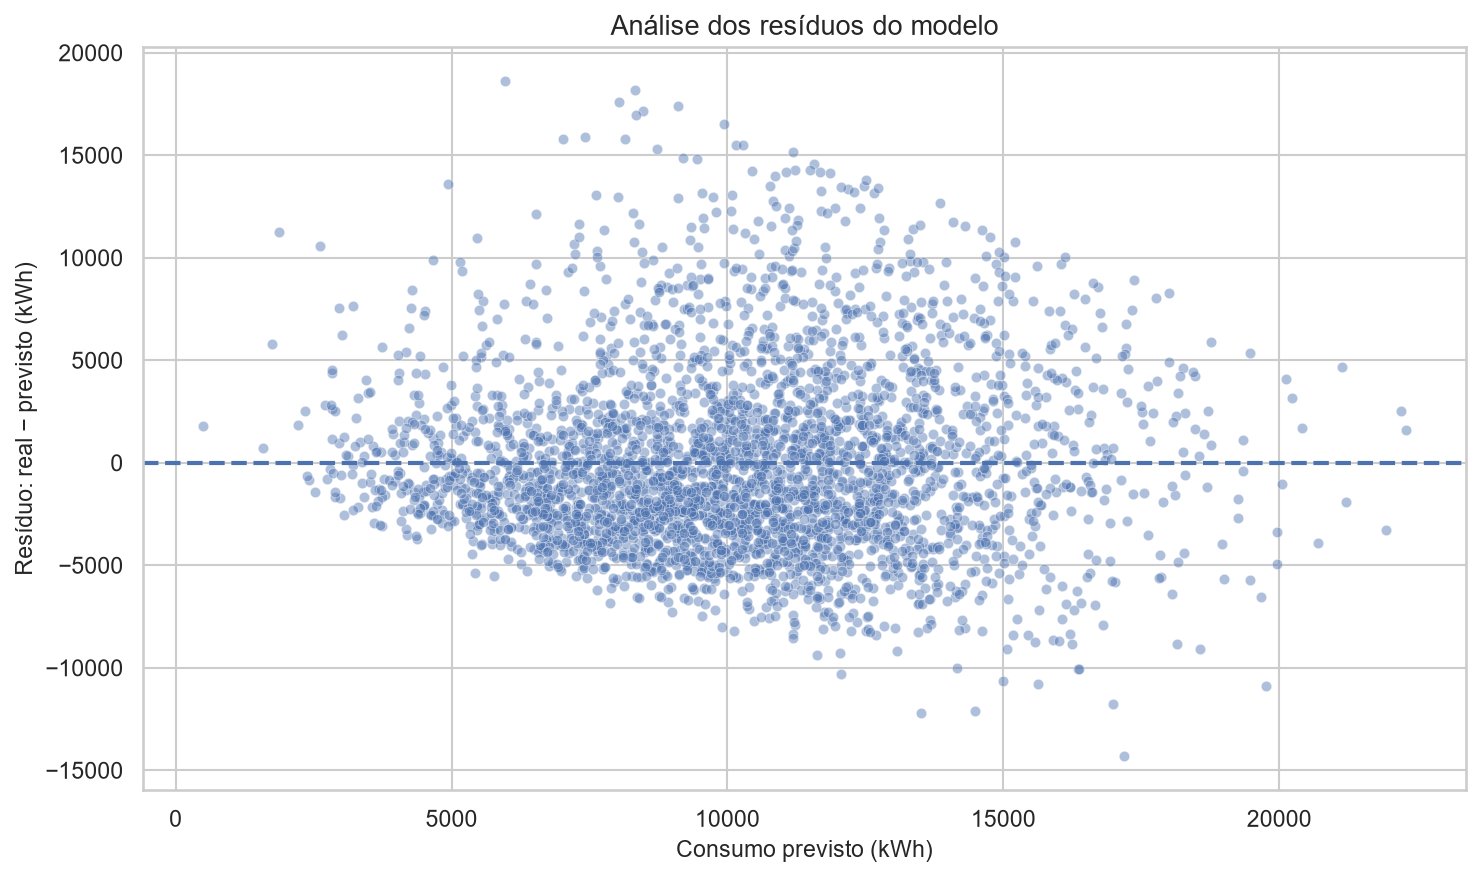
\includegraphics[width=0.85\textwidth]{figuras/04_residuos.png}
	\caption{Distribuição dos resíduos em função dos valores previstos.}
	\label{fig:residuos}
\end{figure}

A análise dos resíduos permite investigar possíveis padrões nos erros de previsão. Em um modelo adequado, espera-se que os resíduos estejam distribuídos aleatoriamente ao redor da linha zero, sem apresentar tendências sistemáticas. A presença de padrões pode indicar limitações na representação da relação entre as variáveis pelo modelo linear.

\section{Análise dos coeficientes}

Os coeficientes estimados representam a variação esperada no consumo de energia elétrica associada ao aumento de uma unidade em cada variável preditora, mantendo as demais constantes. Coeficientes positivos indicam uma relação positiva com o consumo previsto, enquanto coeficientes negativos indicam uma relação negativa.

\begin{figure}[htbp]
	\centering
	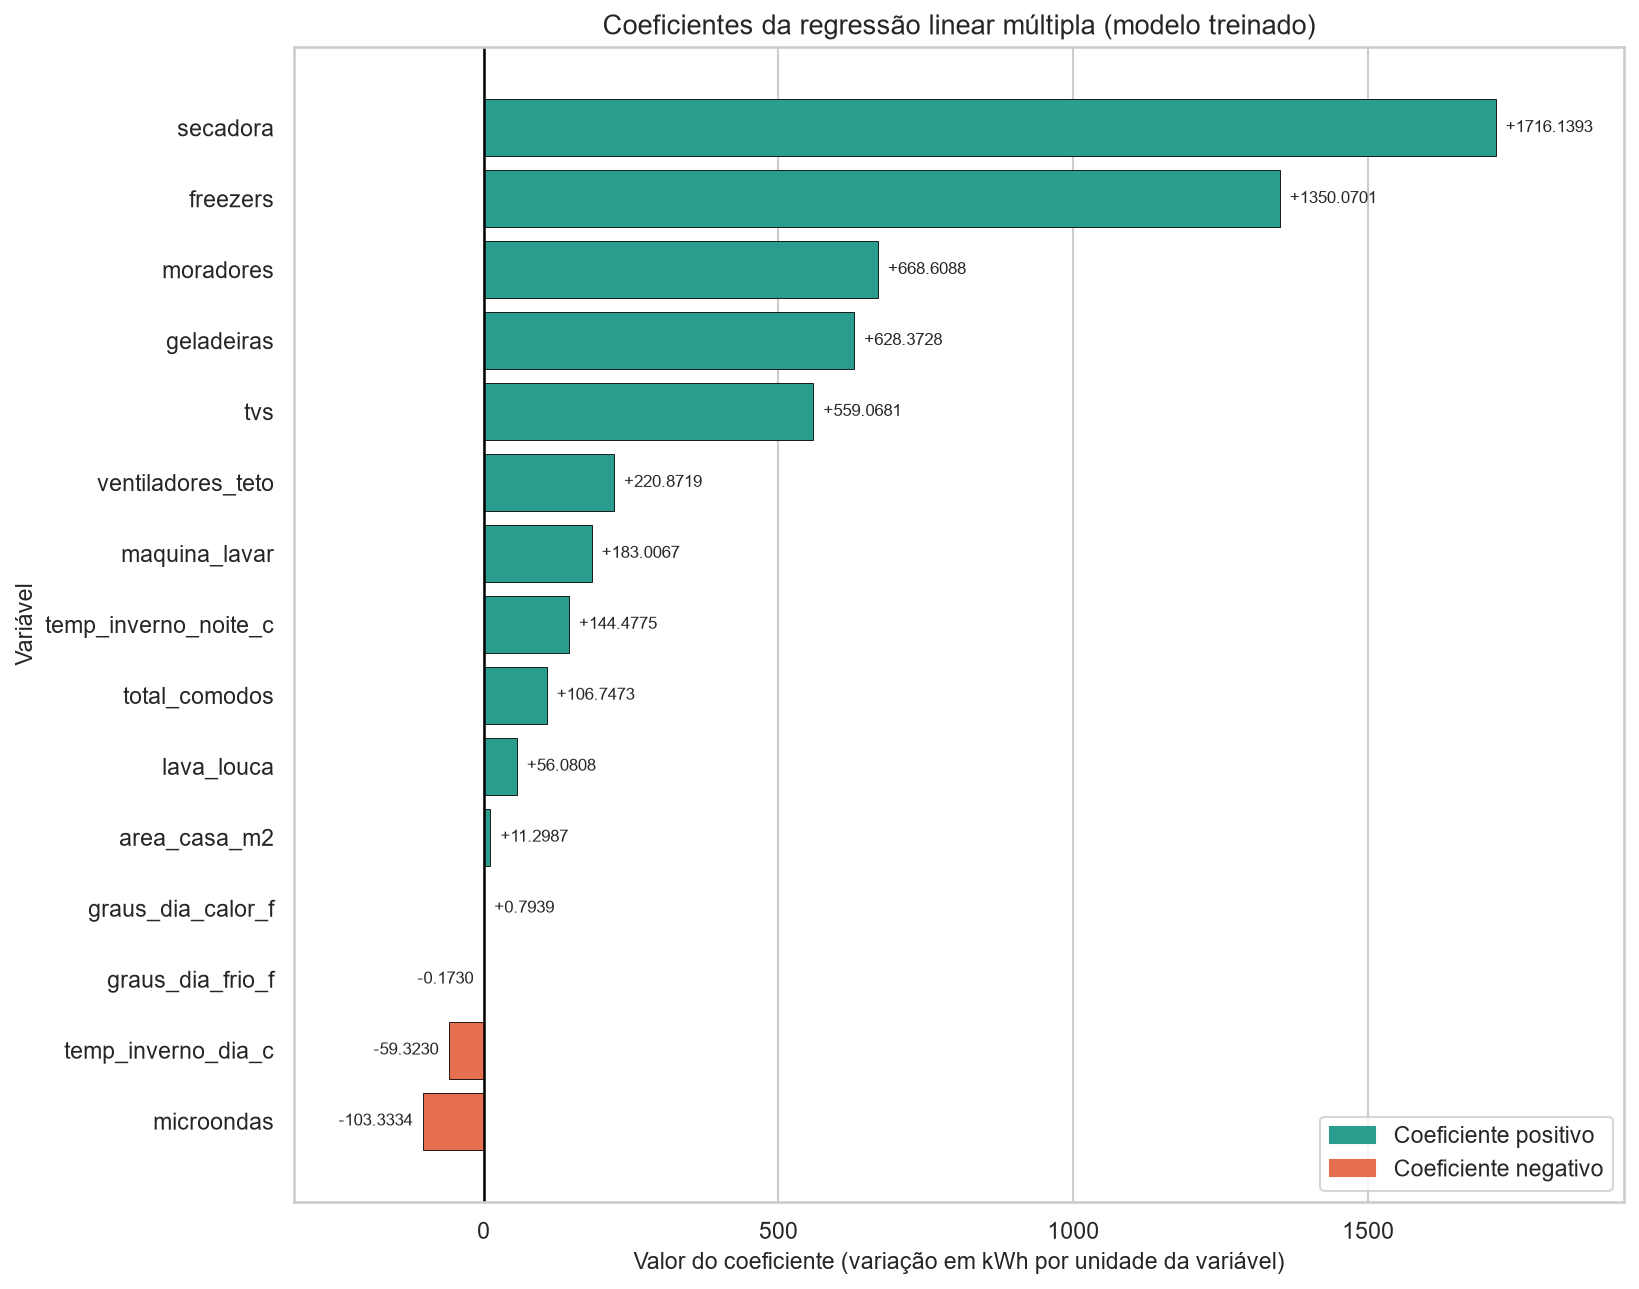
\includegraphics[width=0.95\textwidth]{figuras/05_coeficientes_modelo.png}
	\caption{Coeficientes estimados pela regressão linear múltipla.}
	\label{fig:coeficientes}
\end{figure}

Entre os coeficientes positivos, destacam-se os associados à presença de secadora (1716,1393), à quantidade de freezers (1350,0701) e ao número de moradores (668,6088). Por outro lado, algumas variáveis apresentaram coeficientes negativos, como a temperatura média diurna no inverno (-59,3230) e a quantidade de micro-ondas (-103,3333).

É importante considerar que os coeficientes estão expressos nas unidades originais das variáveis. Portanto, seus valores absolutos não devem ser comparados diretamente como medida de importância, uma vez que as variáveis possuem escalas e unidades diferentes.
